\documentclass{beamer}
\usetheme{Boadilla}

\usepackage[utf8]{inputenc}
\usepackage{graphicx}
\usepackage{epstopdf}
\epstopdfDeclareGraphicsRule{.tif}{png}{.png}{convert #1 \OutputFile}
\AppendGraphicsExtensions{.tif}


\usepackage{booktabs}

\usepackage{rotating}

\usepackage{tikz}
\usetikzlibrary{positioning,shapes}

\title{FSDL Report on Aerial Segmentation}
\author{Fabian Berressem \and Jonathan Schaust}
\date{\today}
\begin{document}
\begin{frame}
\titlepage
\end{frame}

\section{Project Description}

\begin{frame}
\frametitle{Project Description}
\begin{itemize}
\item Task of this project: Segmentation of aerial orthomosaics into six different classes (building, clutter, vegetation, water, ground, car)
\item Given data: 55 aerial photographs with corresponding segmentation and elevation maps (total of 9.7 GB data)
\item Example:
\end{itemize}
\vspace*{0.5cm}
\begin{minipage}{0.65\textwidth}
\centering
\begin{figure}
\fbox{\includegraphics[width=0.45\textwidth]{images/2ef3a4994a_0CCD105428INSPIRE-ortho.png}}
\fbox{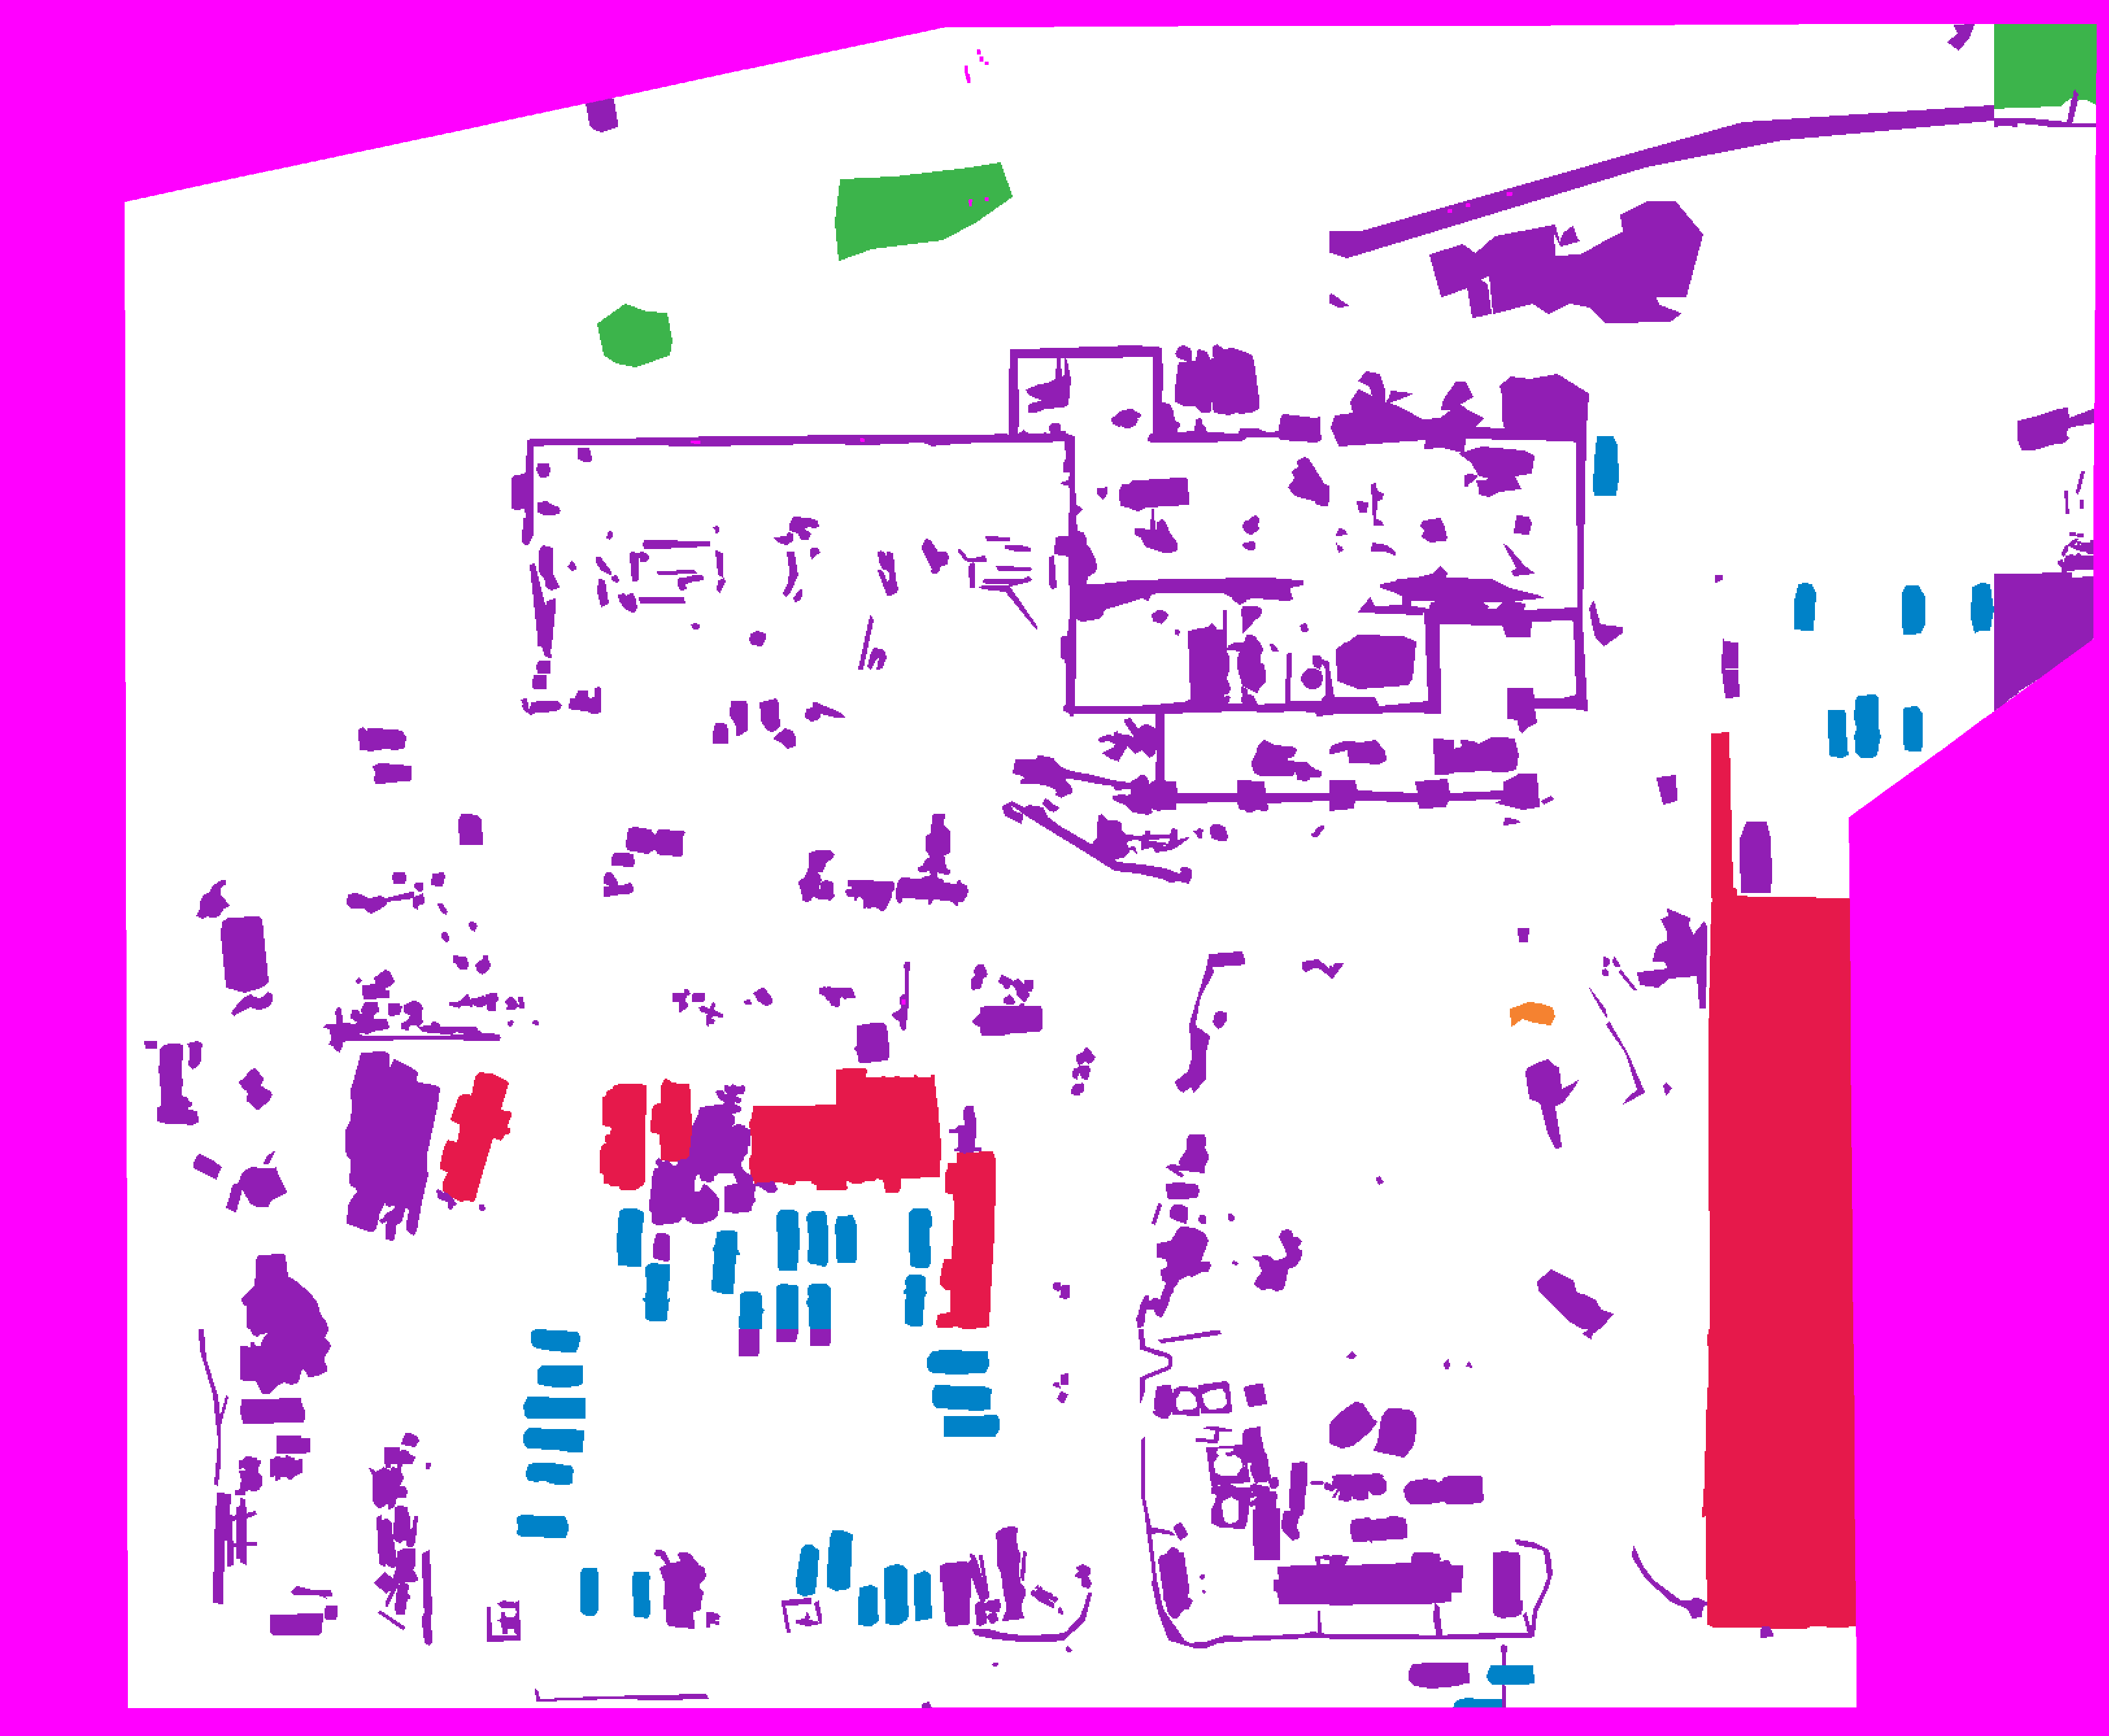
\includegraphics[width=0.45\textwidth]{images/2ef3a4994a_0CCD105428INSPIRE-label.png}}
\end{figure}
\end{minipage}
\hspace*{0.3cm}
\begin{minipage}{0.15\textwidth}
\begin{table}
\centering
\scriptsize
\begin{tabular}{ l|l  }
 Object class & Color\\
 \toprule
 Building & Red  \\ 
 Clutter & Purple  \\
 Vegetation & Green   \\ 
 Water & Orange  \\
 Ground & White   \\ 
 Car & Blue   \\
 Ignore & Magenta
\end{tabular}
\end{table}
\end{minipage}
\end{frame}

\begin{frame}
\frametitle{Data Exploration}
\begin{itemize}
\item Found strong class imbalance (two orders of magnitude)\\
$\Rightarrow$ Possibly have to account for this in loss function
\item Distribution of elevations very similar\\
$\Rightarrow$ Hints at poor quality of labeling, limited information in elevation maps
\end{itemize}
\begin{minipage}{0.49\textwidth}
\begin{figure}
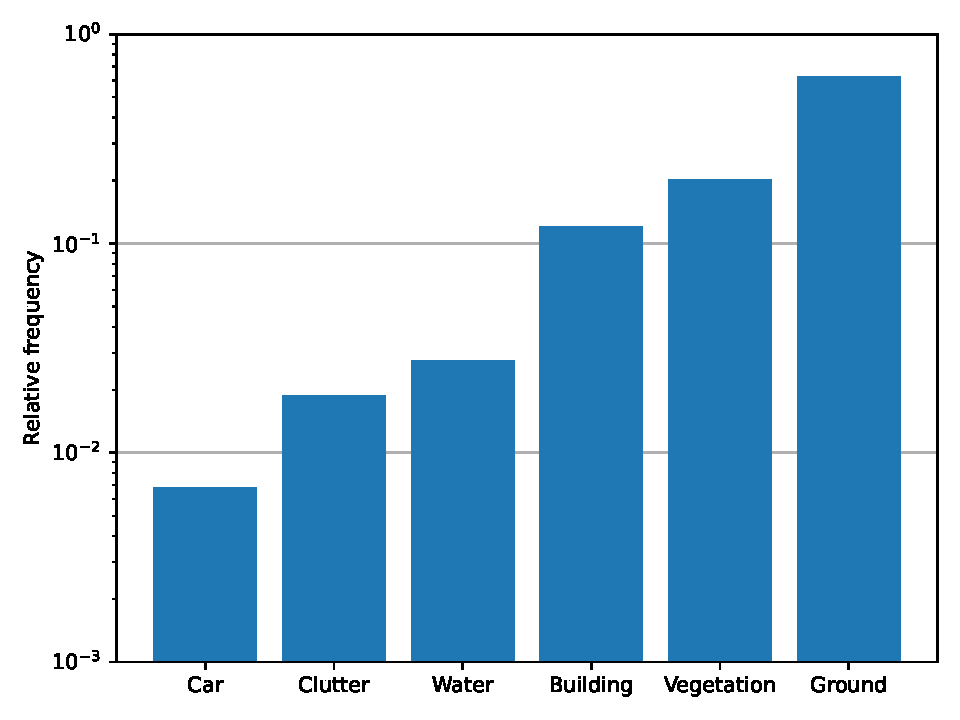
\includegraphics[width=\textwidth]{images/relative_frequency.pdf}
\end{figure}
\end{minipage}
\begin{minipage}{0.49\textwidth}
\begin{figure}
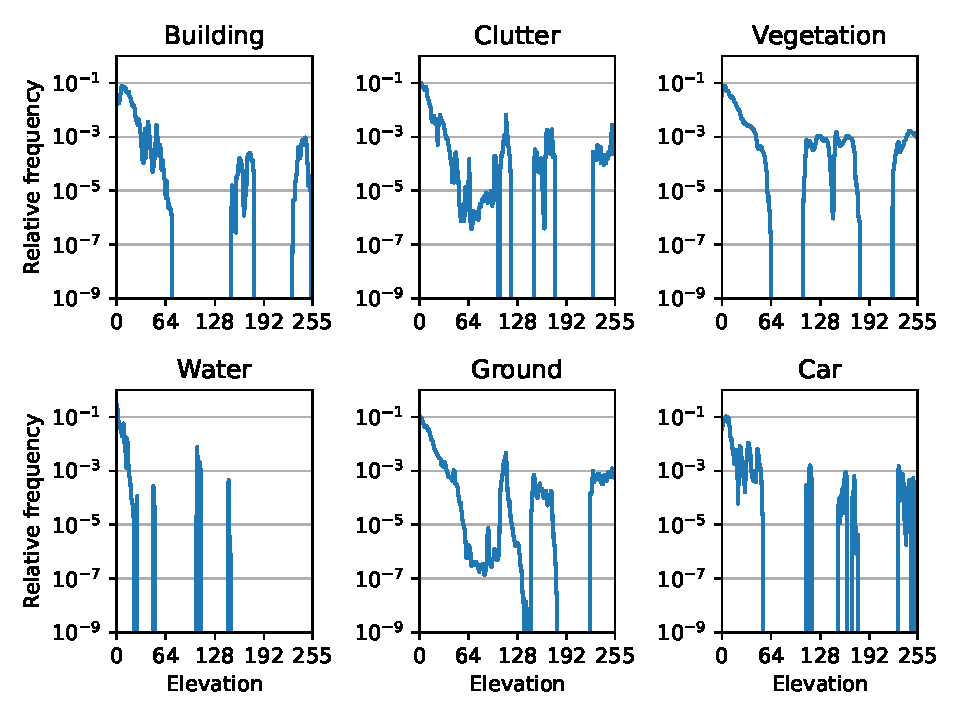
\includegraphics[width=\textwidth]{images/elevation_distribution.pdf}
\end{figure}
\end{minipage}

\end{frame}

\begin{frame}
\frametitle{Approaches}
\begin{itemize}
\item Limited model search to fully convolutional models to allow for different input sizes
\item Implemented additional loss functions such as $F_1$-score, Focal Tversky Loss because of class imbalance
\item Joint learning of segmentation mask and elevation map
\item Implemented learning on adversarial examples using Fast Gradient Signed Method
\end{itemize}
\end{frame}

\begin{frame}
\frametitle{Encountered Problems}
\begin{itemize}
\item Moving objects are ``sliced'' (rather insignificant for prediction)
\item Multiple occurrences of wrong or inconsistent labels
\item Some objects larger than receptive field, context can not propagate properly
\item Images very large, have to be cut into subimages for inference
\item Sometimes blank spots in the pictures, have to be padded\\
$\Rightarrow$ Results in ``artificial'' edges
\end{itemize}
\begin{minipage}{0.3\textwidth}
\begin{figure}
\begin{tikzpicture}
\node(a){\includegraphics[width=\textwidth]{images/9170479165_625EDFBAB6OPENPIPELINE-ortho.png}};
\node at(a.center)[draw, red,line width=0.37*2pt,ellipse, minimum width=0.37*20pt, minimum height=0.37*20pt,rotate=0,yshift=0.37*62pt, xshift=-0.37*14pt]{};
    \node at(a.center)[draw, blue,line width=0.37*2pt,ellipse, minimum width=0.37*30pt, minimum height=0.37*15pt,rotate=0,yshift=0.37*45pt, xshift=0.37*110pt]{};
    \node at(a.center)[draw, blue,line width=0.37*2pt,ellipse, minimum width=0.37*75pt, minimum height=0.37*20pt,rotate=0,yshift=0.37*38pt, xshift=-0.37*32 pt]{};
    \node at(a.center)[draw, green,line width=0.37*2pt,ellipse, minimum width=0.37*10pt, minimum height=0.37*20pt,rotate=0,yshift=-0.37*20pt, xshift=0.37*32pt]{};
\end{tikzpicture}
\end{figure}
\end{minipage}
\begin{minipage}{0.3\textwidth}
\begin{figure}
\begin{tikzpicture}
\node(a){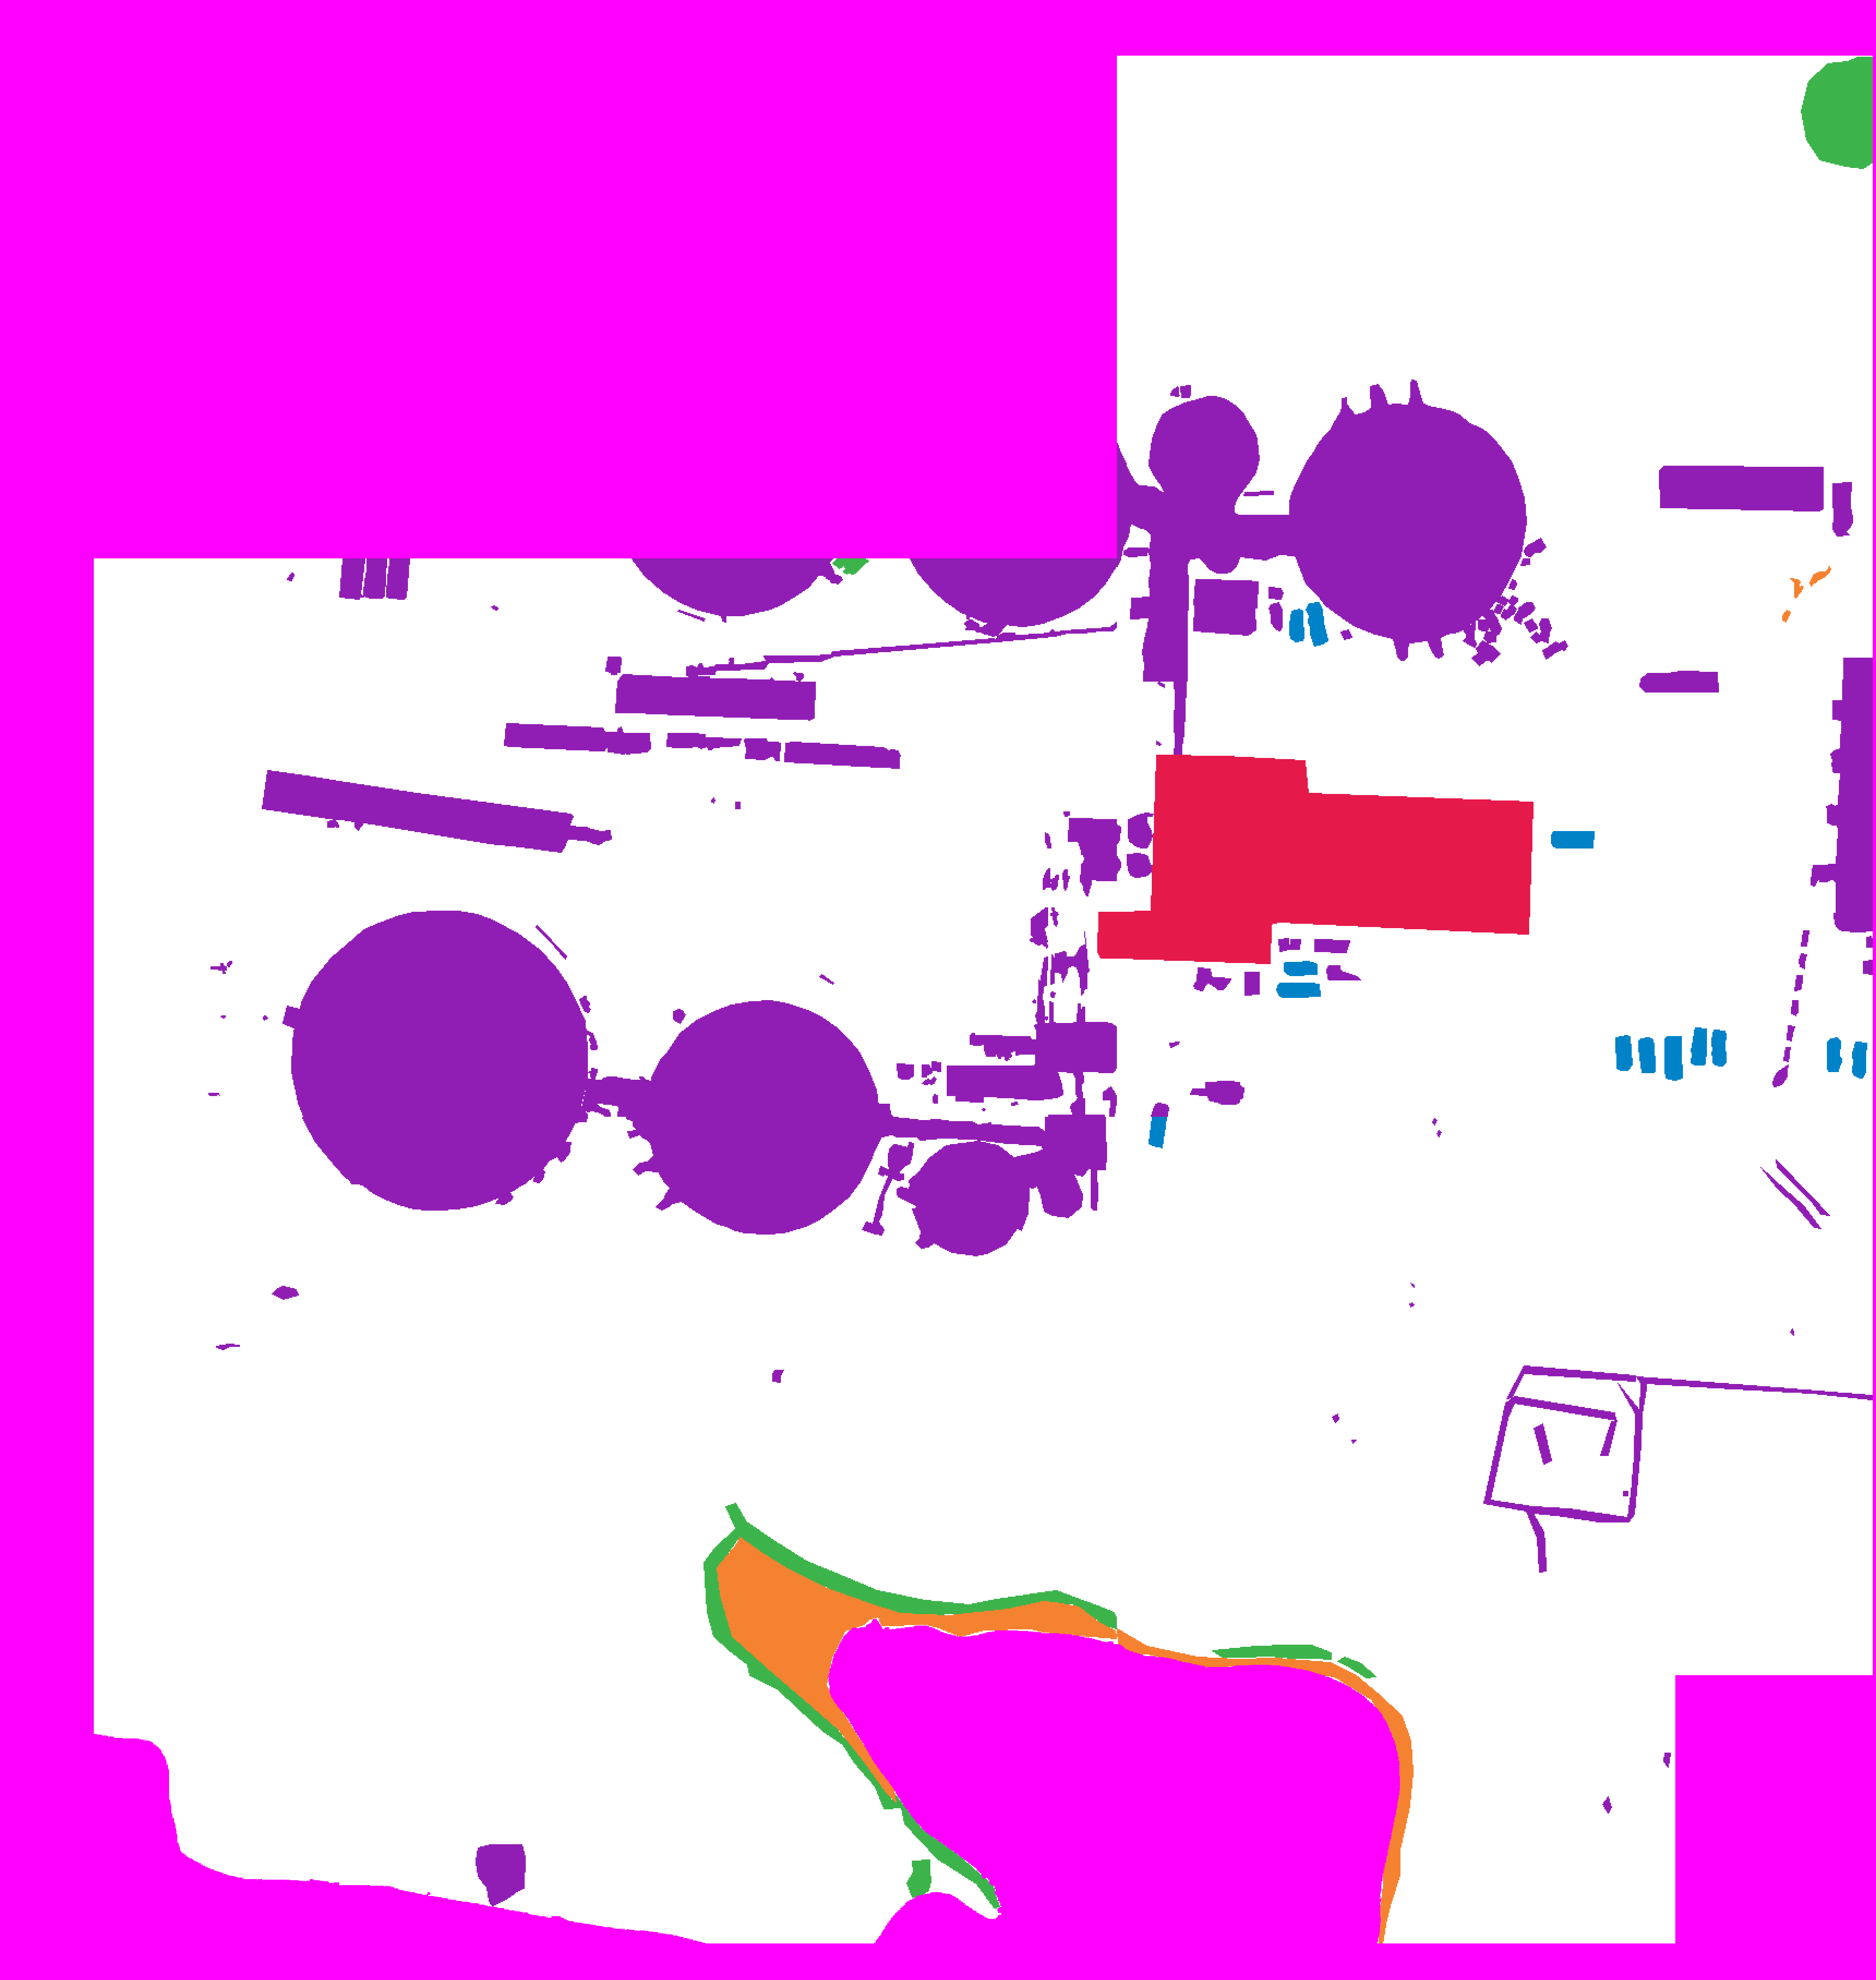
\includegraphics[width=\textwidth]{images/9170479165_625EDFBAB6OPENPIPELINE-label.png}};
\node at(a.center)[draw, red,line width=0.37*2pt,ellipse, minimum width=0.37*20pt, minimum height=0.37*20pt,rotate=0,yshift=0.37*62pt, xshift=-0.37*14pt]{};
    \node at(a.center)[draw, blue,line width=0.37*2pt,ellipse, minimum width=0.37*30pt, minimum height=0.37*15pt,rotate=0,yshift=0.37*45pt, xshift=0.37*110pt]{};
    \node at(a.center)[draw, blue,line width=0.37*2pt,ellipse, minimum width=0.37*75pt, minimum height=0.37*20pt,rotate=0,yshift=0.37*38pt, xshift=-0.37*32 pt]{};
    \node at(a.center)[draw, green,line width=0.37*2pt,ellipse, minimum width=0.37*10pt, minimum height=0.37*20pt,rotate=0,yshift=-0.37*20pt, xshift=0.37*32pt]{};
\end{tikzpicture}
\end{figure}
\end{minipage}
\begin{minipage}{0.3\textwidth}
\begin{figure}
\begin{turn}{90}
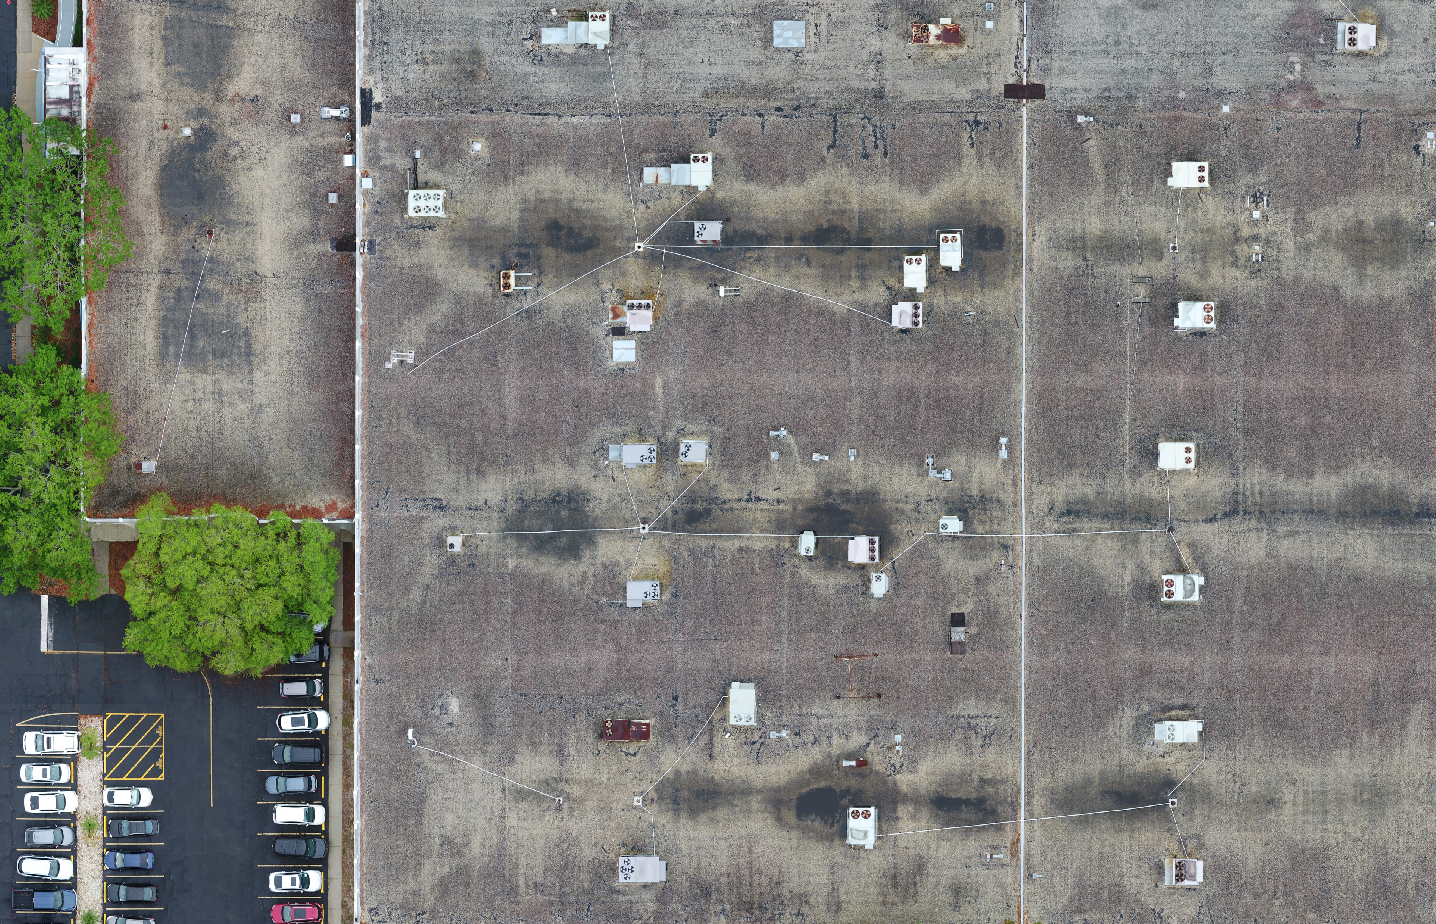
\includegraphics[width=\textwidth]{images/roof.png}
\end{turn}
\end{figure}
\end{minipage}
\end{frame}


\begin{frame}
\frametitle{Solution Strategies}
\begin{itemize}
\item Use a smoothed strided inference to avoid artifacts at boundaries due to cutting images into subimages\\
$\Rightarrow$ Predictions on subimages overlap such that boundary artifacts can be accounted for
\item Use cascading inference to allow for propagation of long-distance context (such as large buildings)\\
$\Rightarrow$ Inference is done successively at different resolutions of the image: first predict on whole image downsampled to input-size of network, then predict on whole image downsampled with increased resolution, merge predictions, \textit{etc}.\\
$\Rightarrow$ Complexity scales as $N^{CI}(\epsilon) \leq N \frac{\epsilon^2}{\epsilon^2 -1}$ with increase of resolution $\epsilon$ and complexity of (strided) prediction $N$
\end{itemize}
\end{frame}


\begin{frame}
\frametitle{Evaluation}
\begin{itemize}
\item Used $F_1$-score on validation set to choose model
\item Performances varied only slightly\\
$\Rightarrow$ Performance is limited more by the task itself rather than model capabilities
\item Chose MobileNetV2 pretrained on ImageNet as encoder with a cross-entropy loss and $\alpha_{elev} = 10$
\item Model was trained on subimages of size $300 \times 300$ while inference was done with subimages of size $4000 \times 4000$ with stride $7$ with smoothing and cascading inference with $\epsilon = 2$
\item Scored $\langle F_1 \rangle_{test} = 0.8496$, which is up $1.6\%$ from the baseline-value of $\langle F_1^{base} \rangle_{test} = 0.8361$
\end{itemize}
\end{frame}

\begin{frame}
\frametitle{Conclusion}
\begin{itemize}
\item Were able to improve on the task of aerial segmentation compared to the baseline
\item Implemented multiple including additional loss functions, different inferences, adversarial training, \textit{etc}.
\item Found severe problems with dataset\\
$\Rightarrow$ To improve on task significantly, quality of dataset \underline{has} to be improved
\end{itemize}
\end{frame}

\end{document}